\documentclass[12pt]{article}
\usepackage[table]{xcolor}
\usepackage[margin=0.9in]{geometry}
\usepackage{amsmath}
\usepackage{graphicx}

\usepackage{setspace}

\usepackage{amssymb}
\usepackage{epstopdf}
\usepackage{inputenc}

\usepackage{dashrule}
\usepackage{float}
\usepackage{hyperref}
\usepackage{url}
\usepackage{mwe}
\usepackage{caption}
\usepackage{multirow}
\usepackage{booktabs}
\usepackage{minted}

\usepackage{helvet}
\renewcommand{\familydefault}{\sfdefault}

\usepackage[backend=biber,style=authoryear-icomp]{biblatex}
\usepackage[toc]{appendix}
\usepackage[acronym]{glossaries}

\addbibresource{references.bib}

\hypersetup{ linktoc=all}
\graphicspath{ {./images/} }


\begin{document}
\title{%
	\bf Biologically Inspired Computing\\ 
    \large - \\
    Training an Artificial Neural Network\\
     using Particle Swarm Optimisation\\
     -\\
     \url{https://www2.macs.hw.ac.uk/~sf52/Bio-Comp-docs/html/index.html}}

\author{
	Sam Fay-Hunt | \texttt{sf52@hw.ac.uk}\\
	Kamil Szymczak | \texttt{ks83@hw.ac.uk}
}

\maketitle
\thispagestyle{empty}
\pagebreak

\tableofcontents
\thispagestyle{empty}
\pagebreak


\setcounter{page}{1}

\section{Introduction}
This report details our rationale when developing our Artificial Neural Network (ANN) and Particle Swarm Optimisation (PSO) implementations, A description of the methodology we employed, and the results from the experiments we performed to gain insight into the factors that can effect the quality of PSO.

Our solution is written in Python, heavily utilising numpy, pandas and the python standard libraries, additionally we made use of matplotlib for plotting graphs and SKlearn to split the data into training and testing sets.
We used an OOP approach to keep the project organised so we could maintain the fairly large codebase, while keeping the ANN and the PSO modules neatly decoupled.
We used jupyter notebooks to demonstrate how to use our codebase, and to present our findings.
We used sphinx to generate documentation of the sourcecode, links to our \href{https://www2.macs.hw.ac.uk/~sf52/Bio-Comp-docs/html/index.html}{documentation} are included throughout this report to help provide context.

\begin{figure}[H]
    \begin{center}
        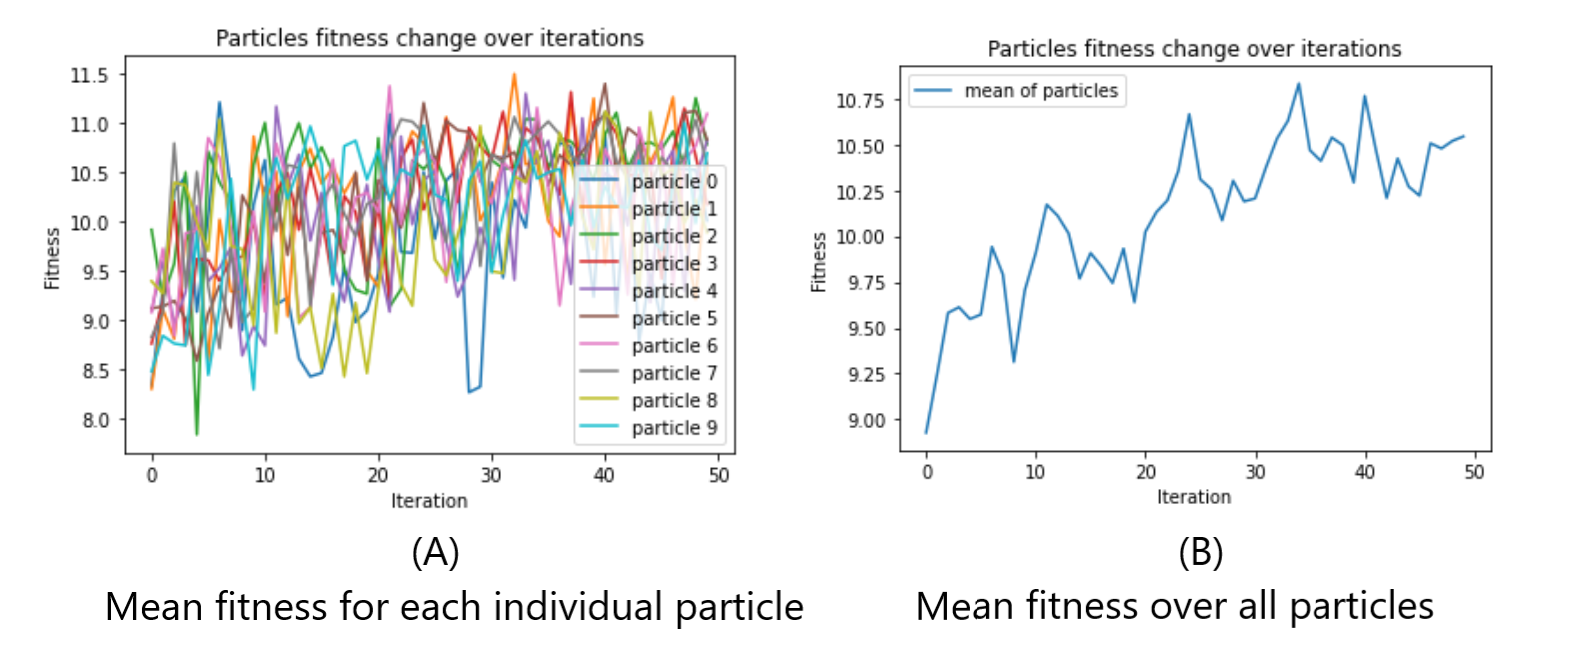
\includegraphics[width=0.85\textwidth]{comples_pso_combined.png} 
    \end{center}
    
    \caption{Learning PSO hyperparameters with PSO for the complex dataset.}
    \label{fig:complexpsolearning}   
\end{figure}

\begin{figure}[H]
    \begin{center}
        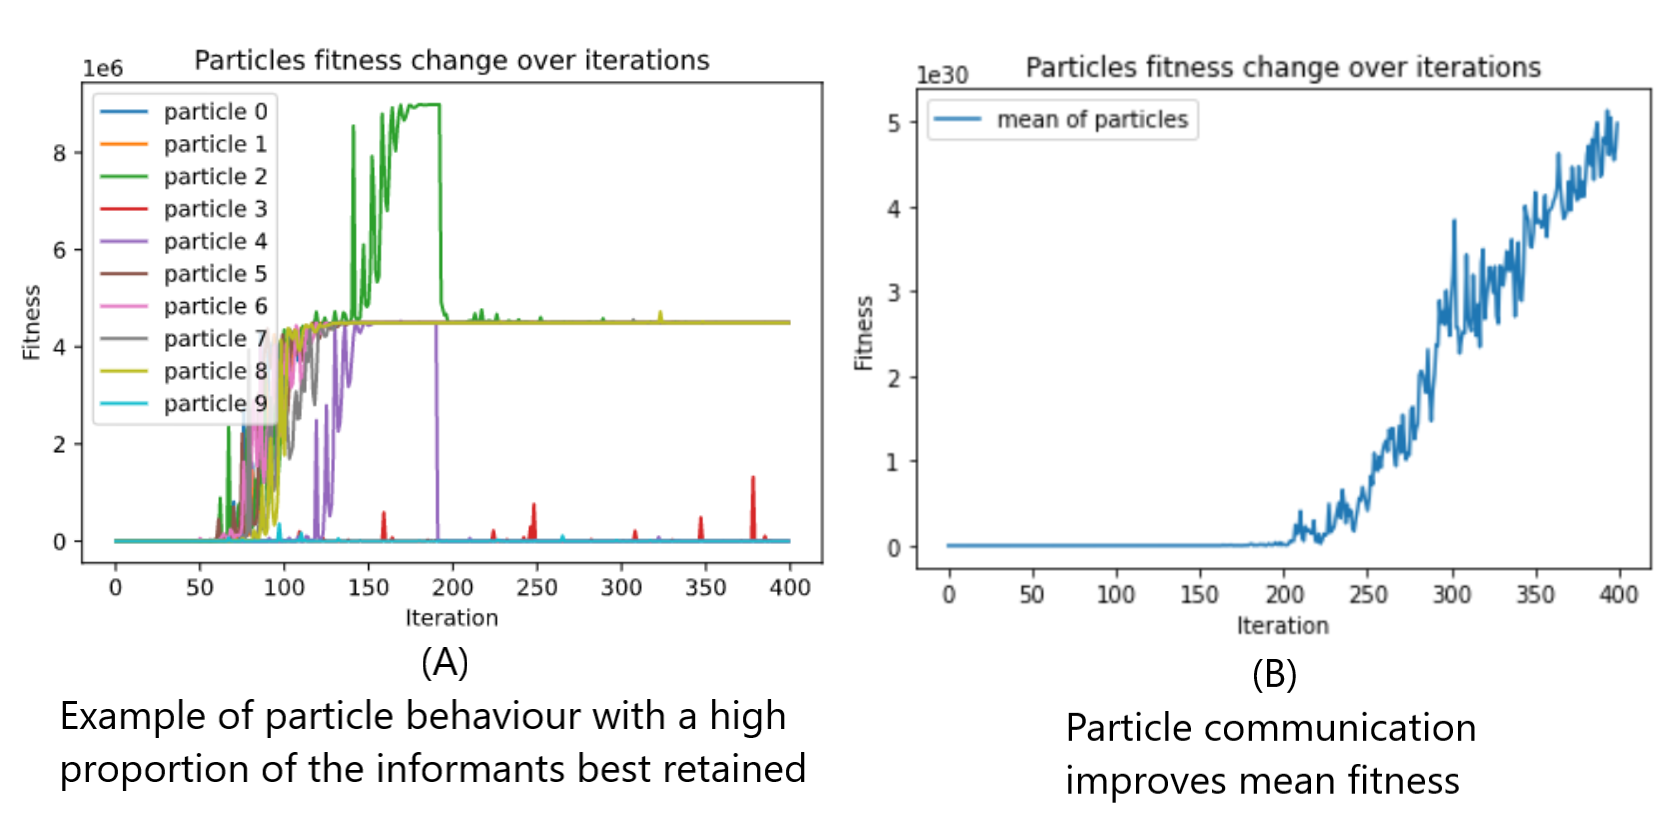
\includegraphics[width=0.8\textwidth]{Examples.png} 
    \end{center}
    
    \caption{Notable examples of PSO hyperparameters effecting fitness}
    \label{fig:ExamplePlots}   
\end{figure}

\section{Development Rationale}
Our rationale was to create 2 submodules: \href{https://www2.macs.hw.ac.uk/~sf52/Bio-Comp-docs/html/Coursework.ANNModel.html}{ANNModel} and \href{https://www2.macs.hw.ac.uk/~sf52/Bio-Comp-docs/html/Coursework.PSO.html}{PSO} that could be used to build a fully connected neural network or perform PSO independently.
We wanted the submodules to be completely decoupled to allow PSO to work on arbitrary Optimisation problems.\\

\noindent~ANNModel is only able to create a fully connected neural network, we made this descision to simplify the process of vectorizing the parameters of the network for optimisation with PSO, this also made converting the vector back into a model easier.

The ANNModel’s design was inspired by TensorFlow \& Keras~\autocite{kerasKerasDocumentationModel,tensorflowModuleTfKeras}, specifically when defining the shape of the neural network. For example you can instantiate the empty network, define the input and result vectors, the layers and then, finally, compile the model.
Once compiled you can perform a \href{https://www2.macs.hw.ac.uk/~sf52/Bio-Comp-docs/html/Coursework.ANNModel.html?highlight=one_pass#Coursework.ANNModel.model.ANN.one_pass}{single pass} on the model with either random weights or activations, biases and weights defined by a vector.\\

\noindent To develop PSO we used the pseudocode from~\autocite{lukeEssentialsMetaheuristicsSet2013}, the PSO class utilises a Particle class to abstract away some complexity.
To use the PSO class define the hyperparameters in the constructor (as described in the \href{https://www2.macs.hw.ac.uk/~sf52/Bio-Comp-docs/html/Coursework.PSO.html?highlight=pso#Coursework.PSO.pswarm.PSO}{documentation}), and then specify the fitness function and search dimensions for PSO. \\

\noindent We created an interface for PSO Called \href{https://www2.macs.hw.ac.uk/~sf52/Bio-Comp-docs/html/Coursework.PSO.html?highlight=optimisable#Coursework.PSO.interface.Optimisable}{Optimisable}, any class that properly implements this interface can be used with our PSO implementation. 
The beauty of this technique is that it allowed us to implement this interface on our PSO class and construct a (PSO) optimiser for our PSO hyperparameters for a specific model shape, for clarity we refer to this outer PSO optimiser as ``meta-PSO'' and the inner PSO optimiser as ``inner-PSO''.

This interface also allowed us to create some wrapper classes(PSOHistory, PSOFittest) that can store detailed data about all the hyperparameter settings of the model being optimised.
Figure~\ref{fig:dimensionVec} shows the definitions of  the hyperparameters and boundaries that our meta PSO algorithm searches over. 

\begin{figure}[h]
    \begin{minted}{python}
        def dimension_vec(self):
            swarm_size = (10, 100)
            informants = (4, 8)
            alpha = (0.01, 2.0)
            beta = (0.01, 2.0)
            gamma = (0.01, 2.0)
            delta = (0.01, 2.0)
            epsilon = (0.01, 2.0)
            return [swarm_size, informants, alpha, beta, gamma, delta, epsilon]
    \end{minted}
    \caption{A list describing the dimensions and boundaries that PSO will search over. See the documentation for more information~\autocite{fay-huntBiologicallyInspiredComputation}.}
    \label{fig:dimensionVec}
\end{figure}


\newpage
\section{Experimentation Methodology}\label{sec:experiment}

As explained in the previous section, we used a method to find good PSO hyperparameters by applying PSO to another PSO that itself tries to optimize our ANN for a defined dataset.
This allowed us to investigate a wide search space of potential optimal hyperparameters for the PSO model that was used to optimize the given ANN.\\

We ran all experiments defined in Table~\ref{tab:ExperimentResults}~on a neural network with only 4 neurons in its hidden layer and 1 neuron in the output layer, while this did make it harder to find the ideal neural network hyperparameters for some functions in some cases the results were surprisingly accurate.
We used mean squared error as the loss function, also we initialise our ANN with activation functions however the activation functions used are learned by PSO.\\

To score the hyperparameters we used a subset of the input data from the and calculated the percentage of correct approximations within a tolerance of $\pm 0.03$.

\noindent\textbf{Experiment steps:}
\begin{enumerate}
    \item Run the Meta\_pso notebook with each dataset and record the resulting vectors representing the ANN \& PSO hyperparameters.
    \item Copy the vectors from Meta\_pso to the evaluation notebook (See Appendix~\ref{app:PSOconf} \& Appendix~\ref{app:ANNconf}).
    \item For each pair of datasets and corresponding vectors from Meta\_pso set the corresponding training/testing data, the decimal places to compare, the PSO, and ANN parameters.
    \item Run the tests and record the results.
\end{enumerate}

\begin{figure}[H]
    \begin{center}
        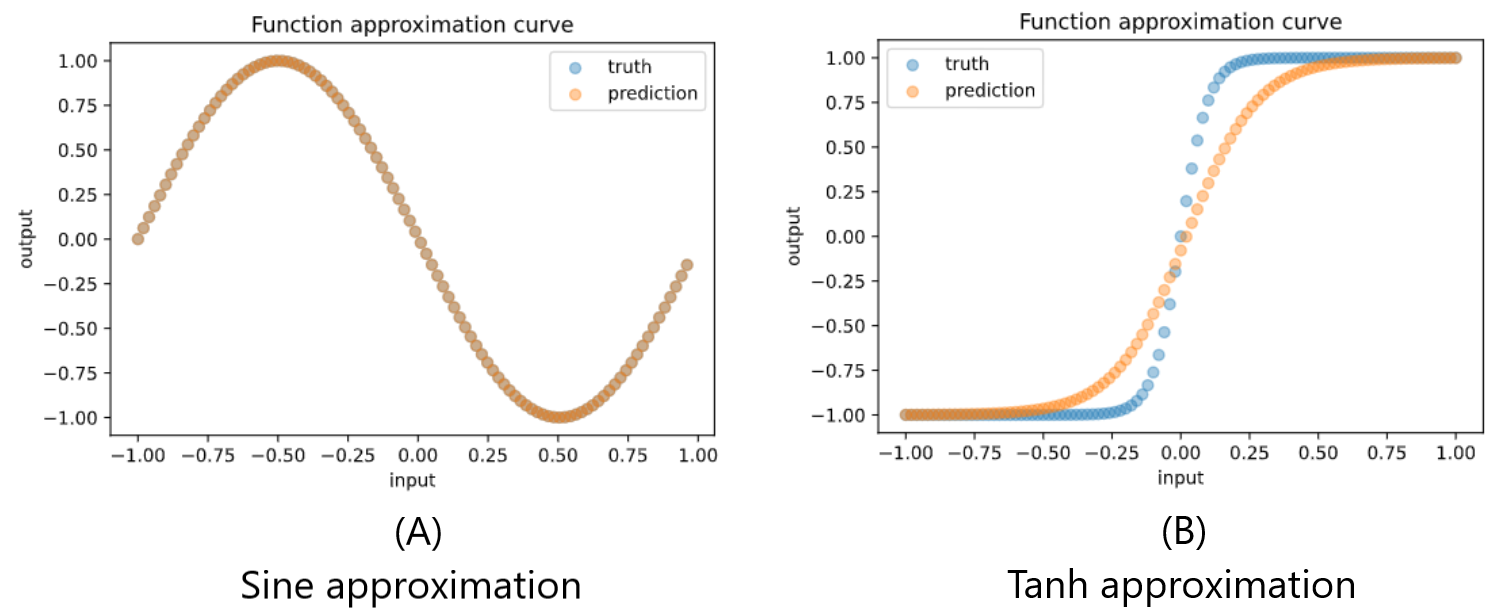
\includegraphics[width=1\textwidth]{approximation_curve_plot.png} 
    \end{center}
    \caption{Visualized function approximation curve\\
    (A) is with an improved neural network architecture, (B) is produced by the network defined in Section~\ref{sec:experiment} }
    \label{fig:approximationCurve}   
\end{figure}

\clearpage
\section{Results}
\begin{table}[H]
    \begin{tabular}{@{}|cl|l|lll|@{}}
    \toprule
    \multicolumn{1}{|l}{}                        & Experiment                                                                                   & Data  & Fitness & Loss  & Score* \\ \midrule
    \multirow{6}{*}{Cubic} & \multirow{2}{*}{\begin{tabular}[c]{@{}l@{}}Best ANN Params\\ meta-PSO\end{tabular}}               & Train & 55 & 0.018 & 15\% \\ \cline{3-6} 
                       &                                                                                                   & Test  & 70 & 0.014 & 15\% \\ \cline{2-6} 
                       & \multirow{2}{*}{\begin{tabular}[c]{@{}l@{}}Best ANN Params\\ (10 runs) mean\end{tabular}}         & Train & 46 & 0.022 & 28\% \\ \cline{3-6} 
                       &                                                                                                   & Test  & 65 & 0.015 & 38\% \\ \cline{2-6} 
                       & \multirow{2}{*}{\begin{tabular}[c]{@{}l@{}}Average from best\\ PSO params (10 runs)\end{tabular}} & Train & 39 & 0.026 & 13\% \\ \cline{3-6} 
                       &                                                                                                   & Test  & 50 & 0.02  & 11\% \\ \bottomrule
    \multirow{6}{*}{Linear} & \multirow{2}{*}{\begin{tabular}[c]{@{}l@{}}Best ANN Params\\ meta-PSO\end{tabular}}               & Train & 10992018104273 & 0.0   & 100\% \\ \cline{3-6} 
                       &                                                                                                   & Test  & 12840847838954 & 0.0   & 100\% \\ \cline{2-6} 
                       & \multirow{2}{*}{\begin{tabular}[c]{@{}l@{}}Best ANN Params\\ (10 runs) mean\end{tabular}}         & Train & 5.635e+32      & 0.0   & 100\% \\ \cline{3-6} 
                       &                                                                                                   & Test  & 3.755e+32      & 0.0   & 100\% \\ \cline{2-6} 
                       & \multirow{2}{*}{\begin{tabular}[c]{@{}l@{}}Average from best\\ PSO params (10 runs)\end{tabular}} & Train & 5.634e+31      & 0.003 & 71\%  \\ \cline{3-6} 
                       &                                                                                                   & Test  & 3.755e31       & 0.003 & 69\%  \\ \bottomrule
                       \multirow{6}{*}{Tanh} & \multirow{2}{*}{\begin{tabular}[c]{@{}l@{}}Best ANN Params\\ meta-PSO\end{tabular}}               & Train & 39 & 0.025 & 49\% \\ \cline{3-6} 
                       &                                                                                                   & Test  & 24 & 0.041 & 38\% \\ \cline{2-6} 
                       & \multirow{2}{*}{\begin{tabular}[c]{@{}l@{}}Best ANN Params\\ (10 runs) mean\end{tabular}}         & Train & 33 & 0.031 & 45\% \\ \cline{3-6} 
                       &                                                                                                   & Test  & 22 & 0.046 & 38\% \\ \cline{2-6} 
                       & \multirow{2}{*}{\begin{tabular}[c]{@{}l@{}}Average from best\\ PSO params (10 runs)\end{tabular}} & Train & 25 & 0.047 & 32\% \\ \cline{3-6} 
                       &                                                                                                   & Test  & 17 & 0.066 & 27\% \\ \bottomrule
  
    \multirow{6}{*}{Sine} & \multirow{2}{*}{\begin{tabular}[c]{@{}l@{}}Best ANN Params\\ meta-PSO\end{tabular}}               & Train & 4212   & 0.0   & 93\% \\ \cline{3-6} 
                       &                                                                                                   & Test  & 24     & 0.0   & 88\% \\ \cline{2-6} 
                       & \multirow{2}{*}{\begin{tabular}[c]{@{}l@{}}Best ANN Params\\ (10 runs) mean\end{tabular}}         & Train & 10.006 & 0.099 & 11\% \\ \cline{3-6} 
                       &                                                                                                   & Test  & 10.02  & 0.1   & 18\% \\ \cline{2-6} 
                       & \multirow{2}{*}{\begin{tabular}[c]{@{}l@{}}Average from best\\ PSO params (10 runs)\end{tabular}} & Train & 9.21   & 0.111 & 8\%  \\ \cline{3-6} 
                       &                                                                                                   & Test  & 8.759  & 0.117 & 9\%  \\ \bottomrule
  
    \multirow{6}{*}{Complex} & \multirow{2}{*}{\begin{tabular}[c]{@{}l@{}}Best ANN Params\\ meta-PSO\end{tabular}}               & Train & 20.17  & 0.05  & 9\%  \\ \cline{3-6} 
                          &                                                                                                   & Test  & 16.05  & 0.062 & 18\% \\ \cline{2-6} 
                          & \multirow{2}{*}{\begin{tabular}[c]{@{}l@{}}Best ANN Params\\ (10 runs) mean\end{tabular}}         & Train & 12.028 & 0.083 & 10\% \\ \cline{3-6} 
                          &                                                                                                   & Test  & 24.834 & 0.04  & 15\% \\ \cline{2-6} 
                          & \multirow{2}{*}{\begin{tabular}[c]{@{}l@{}}Average from best\\ PSO params (10 runs)\end{tabular}} & Train & 11.078 & 0.091 & 8\%  \\ \cline{3-6} 
                          &                                                                                                   & Test  & 14.796 & 0.07  & 4\%  \\ \bottomrule                   
    \multirow{6}{*}{XOR} & \multirow{2}{*}{\begin{tabular}[c]{@{}l@{}}Best ANN Params\\ meta-PSO\end{tabular}}               & Train & 27110227206 & 0.0   & 100\% \\ \cline{3-6} 
                          &                                                                                                   & Test  & 24306553208 & 0.0   & 100\% \\ \cline{2-6} 
                          & \multirow{2}{*}{\begin{tabular}[c]{@{}l@{}}Best ANN Params\\ (10 runs) mean\end{tabular}}         & Train & 77.32       & 0.013 & 100\% \\ \cline{3-6} 
                          &                                                                                                   & Test  & 93.254      & 0.011 & 100\% \\ \cline{2-6} 
                          & \multirow{2}{*}{\begin{tabular}[c]{@{}l@{}}Average from best\\ PSO params (10 runs)\end{tabular}} & Train & 16.716      & 0.102 & 95\%  \\ \cline{3-6} 
                          &                                                                                                   & Test  & 16.023      & 0.134 & 88\%  \\ \bottomrule                   
    \end{tabular}
    \caption{Table of results, showing the scores from the best ANN parameters from meta-PSO, and the mean best scores from an optimiser using the hyperparameters discovered in meta-PSO.}
    \label{tab:ExperimentResults}
\end{table}

\section{Conclusion}

\subsection{Further work}
\textbf{Areas for improvement in the experiment:}
\begin{itemize}
    \item We use a fixed model structure for our neural network during testing, so some functions were far easier to approximate than others.
    \item The fitness function we used was simply 1/loss, this was easy to implement but may have impacted the ability of PSO to escape local maximum. In future a alternative fitness functions should be investigated (perhaps one that scales linearly).
    \item During meta-PSO we only took the mean of 10 inner-PSO runs to evaluate the fitness of each inner-PSO hyperparameter configuration. More would have been better, but impractical in terms of time.
\end{itemize}
From the experimental results we have observed, we feel future experiments should look closer at other fitness evaluation techniques. 
An investigation into different hyperparameter search dimensions for both the ANN model and PSO would be interesting, some hyperparameters were found very quickly and it may be worth investigating if we could freeze those once they are found during optimiser runtime and reduce the search dimensions (careful consideration should be made with getting stuck in local maxima here). 

A proper benchmark suite should be implemented to identify the serious bottlenecks in computation and memory access so we can begin to address them, and run more comprehensive experiments within a reasonable timeframe.
Likewise a unit testing suite would be helpful in idientifying any remaining bugs in this codebase, and may also provide some insight into the performance bottlenecks.

Implementing PSO visualization tools to view how the hyperparameters are affecting the fitness in real-time would provide more insight into what is going on with particles during optimization. 
This information might allow us to identify hyperparameters that tend to result in the particle being caught in local maxima.

\subsection{Discussion}

The best ANN hyperparameters we observed appeared to be a result of running at least 12.5 million different ANN hyperparameter configurations each time we ran meta-PSO in an attempt to optimise the inner-PSO hyperparameters for a given dataset. 
This suggests the highest performing ANN hyperparameters discovered during our search for good PSO hyperparameters were more due to reinitialising PSO so many times than actually finding some really good PSO hyperparameters.


Findings in~\autocite{garcia-nietoWhySixInformants2012,garcia-nietoEmpiricalComputationQuasioptimal2011} indicate that 6 to 8 informants is generally a good number of informants that each particle should have, our own findings support this as seen in Appendix~\ref{app:PSOconf} where the second index in each vector is a float representing the number of informants (when rounded), all have either 6 or 7 informants.


We frequently observed PSO getting stuck in local maxima, this is reflected by the disparity in table~\ref{tab:ExperimentResults} between the 10 run mean results and the results recorded from the best found during meta-PSO. 
Adjusting the proportion of velocity for each particle to retain and jump size helped to break out of these local maxima but also made the results far more erratic.
Meta-PSO found a mean swarm size of 83 particles, this somewhat supports the observation that this is more of a brute force approach by trying many more possible starting points for each PSO we have a higher chance of finding a higher maximum.


We could achieve a significant improvement in fitness, and accuracy in the lower scoring neural networks when we added an appropriate (for the specific function being approximated) number of neurons and layers to the neural network being optimised, however doing so did not guarentee that we would consistenly find those optimal ANN hyperparameters. 
Figure~\ref{fig:approximationCurve} shows a sine function approximation that we found easily with 10 neurons in the hidden layer instead of 4, this had a 100\% accuracy score with 0 tolerance to error at 4 decimal places.


A significant factor that prevented more thorough experments and more comprehensive testing were the performance issues with this implementation, the meta-PSO notebook in some cases would take up to an hour and a half per run even with the extremely conservative settings we chose (See Section~\ref{sec:experiment}).
When plotting the mean fitness over all particles we could notice an upward trend such as in Figure~\ref{fig:complexpsolearning}, however any more than 10 particles and 50 iterations was impractical to run.
The PSO classes run method in particular has substantial room for improvement, we suspect the performance issues are due to memory access bottlenecks but would need to investigate furthure to confirm this.

\pagebreak
\appendix

\section{References}
\printbibliography

\newpage
\section{Additional Material}
\subsection{PSO configuration vectors}\label{app:PSOconf}
\begin{figure}[h]
    \begin{minted}[breaklines]{python}
# Cubic (10 runs) mean fitness: 44.37869624714425
Cubic_pso_config_mean = [91.38785822,  6.52696304,  0.59416449,  0.43559926,  0.29415449, 1.29923762,  0.73352514]

# Linear (10 runs) mean fintess: 1103190071387.8752
Linear_pso_config_mean = [85.37707185,  6.86909089,  0.51382895,  0.9798064,  0.12477974, 0.59493009,  0.89702589]

# Tanh (10 runs) mean fitness: 25.520455427936067
Tanh_pso_config_mean = [55.32621771,  7.52578441,  0.12798331,  0.72531664,  1.08313114, 0.29216353,  1.3627685 ]

# Sine (10 runs) mean fitness: 434
Sine_pso_config_mean = [8.73729926e+01, 7.54895398e+00, 7.33998847e-01, 7.52228076e-02, 2.92737853e-01, 3.09977124e-01, 8.51531051e-01]

# Complex (10 runs) mean fitness: 12
Complex_pso_config_mean = [82.66312781,  5.85540776,  0.62559032,  0.58225519,  0.26541185, 1.38181036,  0.6510299 ]

# Xor (10 runs) mean fitness: 2710748526
Xor_pso_config_mean = [96.15250011,  7.08445513,  0.53364588,  0.62468836,  1.57375821, 1.50229261,  0.17895104]

    \end{minted}
    \caption{Vectors describing our best PSO configurations for the various datasets}
    \label{minted:psoVec}
\end{figure}

\newpage
\subsection{ANN configuration vectors}\label{app:ANNconf}
\begin{figure}[h]
    \begin{minted}[breaklines]{python}
# Cubic Most fit model: 109.50653486975476
Cubic_ann_params = np.array([ 5.3012172, -0.57272851, -0.29479981, 0.80752501, -0.45059291, -0.37421024, -0.75524689, -0.44855557, 0.89593846, 0.21242254, 0.65222056, -0.53284427, -0.79926862, -0.79949714, 0.96237351])

# Linear Most fit model: 10965948279221.076
Linear_ann_params = np.array([ 0.15520314, 0.2222954, 0.47238101, -0.83439247, -0.27726962, 0.11339216, -0.7816949, -0.79196132, -0.3392678, 0.41548984, -0.08055252, 0.12817675, -0.71425698, -0.21576561, -0.7553213 ])

# Tanh Most fit model: 39.38730853575883
Tanh_ann_params = np.array([ 0.09854553, 0.39395654, -0.33737974, -0.12358008, 0.4334227, -0.98235414, -0.99205521, 0.98638961, -0.97515305, 2.33845816, 0.51783499, -0.96708832, -0.9922467, 0.9696207, -0.99365926])

# Sine Most fit model: 4212
Sine_ann_params = np.array([ 0.26515734, 0.7400037, -0.0499965, 0.32639921, 0.03951493, 0.93575309, 0.82658881, 0.95566027, 0.89756768, 3.01482873, -0.62419448, -0.9322514, -0.99330274, -0.85322129, -0.65752741])

# Complex Most fit model: 15.36
Complex_ann_params = np.array([ 5.16794124, -0.50701965, -0.02085653, -0.67915966, -0.56917589, 0.93068562, 0.25302176, 0.92653444, 0.67209426, 0.39299595, -0.75832145, -0.44806736, -0.62409455, 2.26094952, -0.26506833, -0.86461154, 0.31096583, 0.90781783, 0.72454439])

# Xor Most fit model: 27107485189
Xor_ann_params = np.array([-0.13057076, -0.66250843, 0.0122888, -0.4294471, -0.56088656, 0.76634383, 0.95302873, 0.27348615, 0.86272884, 0.79509781, 0.80510636,  0.08453014,  0.86190117, 3.37130705, -0.79043449, 0.74686407, 0.4886179, -0.22842822, 0.69471657])

    \end{minted}
    \caption{Vectors describing our best ANN configurations for the various datasets}
    \label{minted:annVec}
\end{figure}

\end{document}
